\documentclass[12pt]{article}
\usepackage{graphicx}

\begin{document}
	\title{A Sample \LaTeX\ Document}
	\author{Math 300}
	\date{\today}
\maketitle
	
\section{Typing Text}
	Since \LaTeX\ is a markup language, any text we type appears on the page,
	unless it contains one of the nine reserved characters of \LaTeX\, listed below.\\
	
	\noindent
	\verb|\ { } & _ ^ % ~ # |\\
	
	\noindent
	If we want those characters to appear on the page, we must precede them by	a backslash, or, in the special case of the backslash itself, we must use the	command \verb|\verb| .In math mode, we can use the command \verb|\backslash|.
	
	Note that there are three kinds of dash-objects. Hyphens are very short, and are typed the way you would expect, using "-". Dashes, as in the range 1--2, are wider, and are typed using \verb|--|. If you feel a need for a wide---dash, you can use \verb|---|.

\section{Units}
	Lengths in \LaTeX\ can be given in a number of Units.
		
	cm \hspace{10pt} Centimeters
	
	em  \hspace{10pt} The width of the letter M in the current font
	
	ex  \hspace{14pt} The height of the letter x in the current font
	
	in \hspace{17pt} Inches
	
	pc \hspace{15pt} Picas (1pc = 12pt)
	
	pt \hspace{16pt} Points (1in = 72pt)
	
	mm \hspace{7pt} Millimeters
		
\newpage

\section{Space}
The most direct way to make spaces is simply to use the \verb|\hspace| and
\verb|\vspace| commands, for horizontal and vertical space, respectively. Each
takes one argument: a distance specification for the size of the space. The
width or height of the space can be positive {\it or} negative. Note that \verb|\vspace|
can only be used in vertical mode; that is, when you are starting a new para-
graph or starting a float or doing something else that shifts text vertically.
It will not work in a line.

\LaTeX\ also has a number of predefined spaces. To produce a space with
fixed width, and which cannot be used as a line break, you may use the \verb|~|
character. This would typically be used to separate initials of an author,
or in other situations where we don’t want to have a single letter or initial
ending a line. More often, we don’t mind a line break, and want the space
to shrink or grow according to the justification requirements on the line. In
that case we make a standard space using \verb|\| ; backslash-space.

There are wider stretchy spaces available to us: \verb|\quad| and \verb|\qquad|. There
is also a "thin space": \verb|\|,. The following words are separated by a thin space,
a standard space, a quad, and a qquad, respectively.

\vspace{8pt}
	\hspace{90pt} space\,space space\quad space\qquad
	space\\
	
	There are also predefined vertical spaces: \verb|\smallskip \medskip|, and
	\verb|\bigskip|, that behave as their names imply.
	
	There are also some exceptionally stretchy spaces that we can use to
	push text around. For example, the following line is set using the command
	text\verb|\hfill| text. The line below it was set using text\verb|\hfill text\hfill text.|
	
	\noindent text\hfill text
	
	\noindent text\hfill text\hfill text.
	
\noindent	You get the idea: \verb|\hfill| makes enough space to fill the line in question com-
	pletely. If more than one \verb|\hfill| appears on a line, then the two negotiate
	over how much space they each get.
	
\section{Lines and Boxes}
	
	There are a variety of ways to make lines and boxes in \LaTeX\. The most
	basic is to make a horizontal rule using \verb|\hrule|.\hrule
	\newpage
	
	\verb|\hrule| makes a new line, and fills it up with a horizontal line. If you
	don’t want an entire line, you can use \verb|\hrulefill|, as in \hrulefill
	.
	
	\noindent This command works like \verb|\hfill|, but instead of filling with space, it uses a
	horizontal rule to fill the line.
	
	To make a box around some content, you can use the \verb|\framebox| com-
	mand. The framebox command puts a box around its argument, so that
	\verb|\framebox{text}| looks like \framebox{text} . It takes optional width and position ar-
	guments, so that \verb|\framebox[3in][l]{text}| appears as
	
	\noindent \framebox[3in][l]{text}
	.
	
\section{Margins}

This section is mistitled. \LaTeX\ does not really do margins, so much as it
places text. It uses several variables in placing the text, which we can set.
For example, to make the left margin on all even-numbered pages 0.5 inches
wider than the default (which is 1 inch), we would define

\noindent \verb|\evensidemargin=0.5in|.

\noindent A list of the variables we can set and their default values follows.

\noindent
\verb|\evensidemargin|\\
\verb|\oddsidemargin|\\
\verb|\topmargin|\\
\verb|\textwidth|\\
\verb|\textheight|\\
\verb|\parskip|\\
\verb|\baselineskip|


\section{Tables}
Sometimes we need to typeset tables. For example, consider Table 1. Any
resemblance of the numbers in Table 1 to those from any authentic poll is
purely coincidental.

\section{Figures}

We can also put figures into our latex documents. For example, the image in
Figure 1 is found at \verb|http://www.math.wsu.edu/kcooper/M300/sniper.jpg|,

\newpage
\begin{table}
	\begin{center}

\caption{Results from a poll that probably never happened.}
	\begin{tabular}{ ||l|c|| } 
		\hline
		\multicolumn{2}{||l||}{{\it  What is your favorite animal?}}\\
		\hline
		Animal & Percentage of respondents\\
		\hline
		Dog & 43\% \\
		Cat &	44\% \\
		Schwarzenegger & 9\% \\
		We kill animals &	4\% \\
		\hline \hline
	\end{tabular}
\end{center}
\label{table:1}
\end{table}



\noindent but must be converted to encapsulated postscript before it can be included
in this document.

\section{Homemade Commands}

It was the best of ideas. It was the worst of ideas. \LaTeX\ was conceived as
a programming language. This is what makes it harder to process using a
wysiwyg interface, but it also allows us to make our own shortcuts. If you
know that a particular expression will appear repeatedly in your document,
you can make an abbreviation for it, or even a command that allows you to
specify arguments. In our case, the sequence "It was the best of {\it fill in the
blank}. It was the worst of {\it fill in the blank}." is to appear many times in this
section, so we created a command as follows:\\

\noindent
\verb|\newcommand{\dickens}[1]{It was the best of #1.|\\
\verb|It was the worst of #1.}|\\
	
\noindent This command takes one argument, which appears wherever a \verb|#1| appears
in the text for the command. Thus, to typeset "It was the best of examples.
It was the worst of examples.", we need only to type \verb|\dickens{examples}|.

\section{Citations and References}
In technical documents there are many references to typographical objects
from the document, and citations of materials from outside the document.
\TeX\ \cite{ref1} [1] and \LaTeX\ \cite{ref2}[2] lets us keep track of those citations by name, rather
than number. Using the "thebibliography" environment gives us automatic

\begin{figure}
	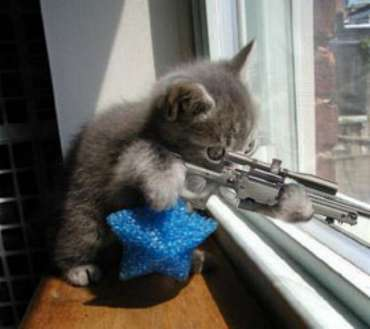
\includegraphics[width=\textwidth]{sniper.jpg}
	\caption{Cats take vengeance on 4\% of respondents \cite{ref3}[3]. }
\end{figure}

\noindent numbering of our references, while associating those numbers with names,
so that we can refer to the references using the \verb|\cite| command. Likewise,
for internal references, such as those to Figure 1, we can assign labels to
a counter using the \verb|\label| command, and refer to them using the \verb|\ref|
command.
\bibliographystyle{plain}
\bibliography{doc.bib}
\end{document}